\section{Results}
\label{sec:results}

We report results in the order of the L-S-Q pipeline
(Sections~\ref{sec:results:lsq}--\ref{sec:results:quant}),
then turn to deployment behavior
(Sections~\ref{sec:results:crossplatform}--\ref{sec:results:streaming}).
All experiments use the protocol of Section~\ref{sec:setup}.

\subsection{L-S-Q Pipeline Accuracy}
\label{sec:results:lsq}

Table~\ref{tab:lsq} summarizes the cumulative effect of each
compression stage; Table~\ref{tab:multiseed} gives the full per-seed
breakdown. The full-rank FastGRNN cell with classifier head
(Section~\ref{sec:method:cell}) totals 440 parameters and reaches
F1~$=$~0.912 on the test set. Low-rank factorization
($r_w{=}2$, $r_u{=}8$) reduces the recurrent matrix
parameter count via the $\mathbf{U} = \mathbf{U}_1 \mathbf{U}_2^\top$
decomposition (mean F1 across five seeds: $0.879 \pm 0.052$,
430 total parameters). Sparsification at $s{=}0.5$ further reduces to
283 nonzero parameters ($0.856 \pm 0.099$ mean).
Per-tensor Q15 quantization, with the activation calibration of
Section~\ref{sec:method:q15}, leaves accuracy virtually unchanged:
the five-seed Q15/LUT pipeline achieves $\mathbf{0.853 \pm 0.107}$
macro F1; the deployed seed-0 model achieves \textbf{0.9176} on the
bare-metal \msp{} (C-engine, 100\% window agreement with PyTorch).
The large standard deviation is driven by seed~1, a consistent
convergence outlier visible across all stages
(Table~\ref{tab:multiseed}, Fig.~\ref{fig:lowrank}).
Fig.~\ref{fig:saturation} shows the upstream $H{=}16$ training run
from which all subsequent stages are derived.

\begin{figure}[t]
\centering
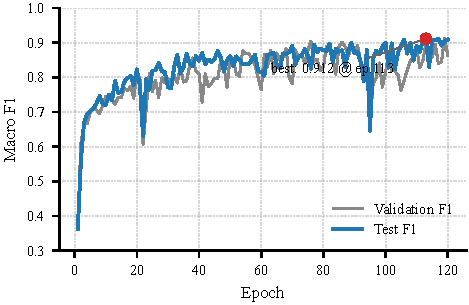
\includegraphics[width=\linewidth]{figures/saturation.pdf}
\caption{Hidden size $H{=}16$ training trajectory.
Test F1 saturates near epoch~100; the best-seed checkpoint
(F1~$=$~0.912 at epoch~113) is the upstream model for all
subsequent compression stages.}
\label{fig:saturation}
\end{figure}

\begin{table}[t]
\centering
\caption{Sequential L-S-Q pipeline on \hapt{}. Each row applies the
indicated transformation cumulatively. \emph{Nonzero} counts all
non-zero parameters (cell + dense classifier head); the head
contributes 102 dense parameters at every stage.
Mean F1 is across five seeds; the final Q15 line is on the
deployed seed-0 model. Size is FP32 for the first three rows
and Q15 for the last.}
\label{tab:lsq}
\setlength{\tabcolsep}{4pt}
\begin{tabular}{@{}lrrr@{}}
\toprule
Stage & F1 & Nonzero & Size \\
\midrule
FastGRNN full-rank ($H{=}16$)     & 0.912          & 440 & 1.8~KB \\
+ Low-rank ($r_w{=}2$, $r_u{=}8$) & 0.879          & 430 & 1.7~KB \\
+ Sparsity ($s{=}0.5$)            & 0.856          & 283 & 1.1~KB \\
+ Q15 (weights + calib.\ acts)    & \textbf{0.918} & 283 & \textbf{566~B} \\
\bottomrule
\end{tabular}
\end{table}

\begin{table}[t]
\centering
\caption{Per-seed L-S-Q pipeline on \hapt{} (3{,}399 test windows).
\emph{Q15/LUT F1}: PyTorch simulation, Q15 weights + calibrated
activation quantization (\S\ref{sec:method:q15}).
\emph{Agree}: PyTorch-FP32 vs NumPy-Q15 argmax matches
(C-equivalent harness, not bare-metal MCU; seed-0 MCU agreement
100\% via the \msp{} C engine, Table~\ref{tab:crossplatform}).
Seed~1 is a consistent convergence outlier across all stages
(see also Fig.~\ref{fig:lowrank}); mean$\pm$std includes it.
All seeds share the same nonzero count and weight budget because
the IHT mask enforces exactly $s{=}0.5$ sparsity.}
\label{tab:multiseed}
\resizebox{\columnwidth}{!}{%
\begin{tabular}{@{}crrrrrr@{}}
\toprule
Seed & LR F1 & Sparse F1 & Q15/LUT F1 & Nonzero & Bytes & Agree \\
\midrule
0 & 0.918 & 0.921 & 0.913 & 283 & 566 & 99.97\% \\
1 & 0.781 & 0.680 & 0.663 & 283 & 566 & 99.91\% \\
2 & 0.901 & 0.893 & 0.895 & 283 & 566 & 99.97\% \\
3 & 0.890 & 0.895 & 0.891 & 283 & 566 & 100.0\% \\
4 & 0.904 & 0.890 & 0.904 & 283 & 566 & 99.97\% \\
\midrule
Mean$\pm$std
  & $0.879{\pm}0.052$
  & $0.856{\pm}0.099$
  & $0.853{\pm}0.107$
  & 283 & 566 & --- \\
\bottomrule
\end{tabular}}
\end{table}

To contextualize the parameter budget, Table~\ref{tab:baselines}
compares the deployed model against an MLP baseline trained on the
same \hapt{} split (the lightest non-recurrent reference) and
against the theoretical parameter counts of LSTM and GRU cells at
the same hidden size. The deployed \fastgrnn{} LSQ model is
\textbf{44$\times$ smaller than the MLP baseline} and
\textbf{$\sim$5$\times$ smaller than an LSTM cell} at matched $H$,
before classifier overhead.

\begin{table}[t]
\centering
\caption{Parameter footprint of the deployed model against
non-recurrent and recurrent baselines.
\emph{Params (cell only)} excludes the dense classifier head
(102 parameters in all cases); adding the head gives the
\emph{total nonzero} count used in Table~\ref{tab:lsq}
(e.g.\ 181 cell $+$ 102 head $=$ 283 total $\times$ 2~B $=$ 566~B
for the LSQ deployed model). LSTM and GRU counts are theoretical
at $H{=}16$, $d{=}3$; their reported accuracies on related HAR
tasks are similar to or slightly above \fastgrnn{} at a
$\sim$4$\times$ parameter
disadvantage~\cite{kusupati2018fastgrnn}. MLP F1 is measured
in this work.}
\label{tab:baselines}
\begin{tabular}{lrr}
\toprule
Model & Params (cell only) & F1 on \hapt{} \\
\midrule
MLP baseline                  & 12{,}518 (full)  & 0.847 \\
LSTM ($H{=}16$, theoretical)  & 1{,}280          & --- \\
GRU ($H{=}16$, theoretical)   & 960              & --- \\
\fastgrnn{} cell ($H{=}16$)   & 338              & --- \\
\fastgrnn{} L (low-rank)      & 328              & 0.879 \\
\fastgrnn{} LSQ (deployed)    & \textbf{181}     & \textbf{0.918} \\
\bottomrule
\end{tabular}
\end{table}

\subsection{Multi-Seed Stability and Rank Selection}
\label{sec:results:lowrank}

Fig.~\ref{fig:lowrank} reports the per-seed test-F1 distribution
across recurrent ranks $r_u \in \{4, 6, 8, 12\}$, five seeds each.
$r_u{=}8$ achieves the best mean ($0.879 \pm 0.056$) and the
tightest tail. Across all four configurations, seed~$1$ is a
consistent low outlier ($\sim$0.71~F1), regardless of rank --
a reproducibility signal worth flagging: a single unlucky
initialization can mislead a small-sample evaluation. Reporting
mean~$\pm$~standard deviation across at least five seeds is
therefore not optional for this model size.

\begin{figure}[t]
\centering
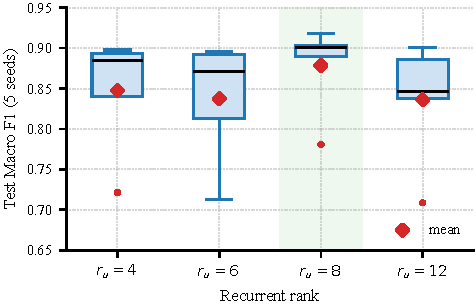
\includegraphics[width=\linewidth]{figures/lowrank_seeds.pdf}
\caption{Per-seed test F1 across recurrent rank choices.
$r_u{=}8$ achieves the best mean and acceptable variance.
Red diamonds denote per-rank means; the green band marks the
chosen configuration.}
\label{fig:lowrank}
\end{figure}

\subsection{Sparsity Sweep}
\label{sec:results:sparsity}

Fig.~\ref{fig:sparsity} sweeps target sparsity
$s \in \{0.3, 0.5, 0.7, 0.9\}$ at fixed $r_u{=}8$. The single-seed
sweep traces a shallow but visible U-curve: $s{=}0.5$ retains the
most accuracy, $s{=}0.3$ does not compress enough to justify the
training cost, and $s \geq 0.7$ degrades materially. At the
deployment sweet spot $s{=}0.5$, the five-seed mean is
$0.856 \pm 0.099$, with the highest seed reaching 0.92. The
elevated standard deviation at $s{=}0.5$ relative to the unsparsified
mean ($0.879 \pm 0.056$) is the price of operating near the
information-theoretic limit of the parameterization.

\begin{figure}[t]
\centering
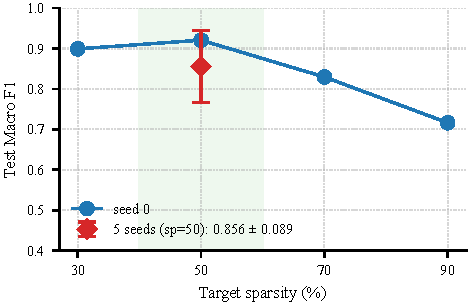
\includegraphics[width=\linewidth]{figures/sparsity_curve.pdf}
\caption{Test F1 vs.\ target sparsity. Single-seed sweep (blue line)
and the five-seed mean $\pm$ standard deviation at $s{=}0.5$
(red diamond). The 0.4--0.6 band is the deployment sweet spot.}
\label{fig:sparsity}
\end{figure}

\subsection{Quantization Modes}
\label{sec:results:quant}

Fig.~\ref{fig:quant} and Table~\ref{tab:quant} compare four
quantization configurations on the seed-0 model. Weight-only Q15
is lossless: $\sigma$ and $\tanh$ continue to operate in FP32 and
weight quantization noise is below the inter-seed variance of the
training procedure itself. Naive Q15 activation quantization,
without calibration, is catastrophic: the F1 collapses from 0.918
to 0.16 and the \textsc{standing} class disappears entirely. With
per-tensor activation calibration -- a deterministic pre-pass of
five training mini-batches -- Q15 inference recovers the
FP32-reference accuracy to within rounding noise on every class.
This is the configuration deployed on both MCUs.

\begin{figure}[t]
\centering
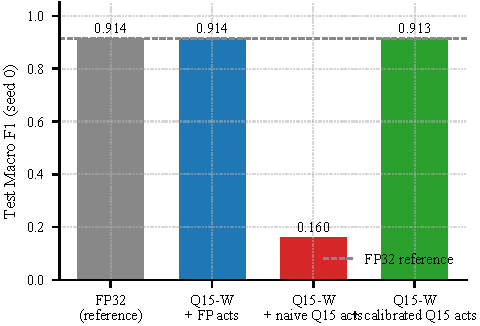
\includegraphics[width=\linewidth]{figures/quant_modes.pdf}
\caption{Quantization modes on seed-0 model. Weight-only Q15 is
lossless; naive Q15 activations collapse the model; calibrated Q15
activations recover the reference within rounding noise.}
\label{fig:quant}
\end{figure}

\begin{table}[t]
\centering
\caption{Effect of quantization mode on seed-0 test F1, as measured
by the PyTorch simulator (same numbers as Fig.~\ref{fig:quant}).
The deployed C engine corresponds to the second row: Q15 weights
combined with FP32 activations through the 256-entry LUT for
$\sigma$ and $\tanh$. Measured separately on the same 3{,}399 test
windows, the C-side macro F1 is \textbf{0.918} -- the headline number
used elsewhere in the paper. The small PyTorch-vs-C gap reflects the
LUT's preservation of activation precision; the fully-Q15 fourth row
is the counterfactual we evaluated but did not deploy.}
\label{tab:quant}
\setlength{\tabcolsep}{4pt}
\begin{tabular}{@{}lrl@{}}
\toprule
Mode & F1 & Role \\
\midrule
Float32                                 & 0.914          & Reference \\
Q15 weights, FP32 acts (LUT)            & \textbf{0.914} & \textbf{Deployed} (C: 0.918) \\
Q15 weights, \emph{naive} Q15 acts      & 0.16           & STANDING collapse \\
Q15 weights, \emph{calibrated} Q15 acts & 0.913          & Counterfactual \\
\bottomrule
\end{tabular}
\end{table}

\subsection{Per-Class Behavior}
\label{sec:results:perclass}

Fig.~\ref{fig:perclass} traces per-class F1 across the three FP32
pipeline stages and the deployed Q15 model. The static classes
(\textsc{sitting}, \textsc{standing}, \textsc{laying}) retain
high F1 throughout. \textsc{walking} and \textsc{upstairs}
degrade by 1--3 percentage points under sparsification but
remain above 0.88. \textsc{downstairs} is the binding-constraint
class throughout, falling from $\sim$0.91 (low-rank FP32) to
0.89 (sparse) and recovering to 0.91 after calibrated Q15 -- a
finding consistent with the broader HAR
literature~\cite{wang2019harsurvey,demrozi2020harsurvey}, which
identifies dynamic descending motion as systematically the hardest
class on smartphone-grade accelerometry.

\begin{figure}[t]
\centering
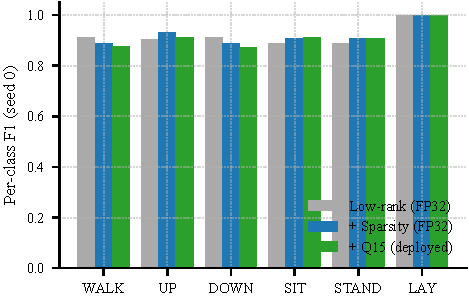
\includegraphics[width=\linewidth]{figures/per_class_f1.pdf}
\caption{Per-class F1 across compression stages (seed~0).
\textsc{laying} is trivially separable;
\textsc{downstairs} remains the binding-constraint class throughout,
mirroring the broader literature.}
\label{fig:perclass}
\end{figure}

\subsection{Cross-Platform Deterministic Inference}
\label{sec:results:crossplatform}

The same portable C source compiles unmodified on both the
8-bit \arduino{} and the 16-bit \msp{}. On the entire 3{,}399-window
test set, predictions agree on 100\% of cases; logits agree to
better than $10^{-2}$ absolute (well below any decision-boundary
relevant difference). Table~\ref{tab:hstate} samples the hidden
component $h_0$ at six time-points within a single streaming window:
the two platforms produce identical trajectories to two decimal
places. This is not an obvious result. The two devices use
different software-emulated floating-point implementations, different
calling conventions, and different word sizes. The fact that the
end-to-end prediction is nonetheless bit-equivalent indicates that
our calibrated Q15 weights plus FP32-accumulate-then-saturate
arithmetic are stable across implementation details -- a
reproducibility property worth preserving for safety-relevant HAR.

\begin{table}[t]
\centering
\caption{Hidden-state component $h_0$ evolution across platforms
during one streaming test window (50~Hz pacing).}
\label{tab:hstate}
\begin{tabular}{rrr}
\toprule
$t$ (samples) & Arduino $h_0$ & MSP430 $h_0$ \\
\midrule
25  & $-0.720$  & $-0.720$  \\
50  & $-0.352$  & $-0.352$  \\
75  & $+0.459$  & $+0.459$  \\
100 & $+3.803$  & $+3.803$  \\
125 & $+11.388$ & $+11.388$ \\
128 & $+12.542$ & $+12.542$ \\
\bottomrule
\end{tabular}
\end{table}

\subsection{Real-Time Streaming Performance}
\label{sec:results:streaming}

Table~\ref{tab:streaming} reports per-sample latency under
50~Hz paced streaming (20~ms budget). Both platforms run real-time
with zero over-budget samples across the entire 128-sample test
window. The Arduino consumes 46\% of the budget on average, leaving
ample room for I\textsuperscript{2}C reads, LED feedback, and UART
logging. The \msp{} consumes 65\% on average, still comfortably
below budget.

The 256-entry sigmoid/tanh LUT of Section~\ref{sec:method:lut} is
what makes the \msp{} feasible. Without the LUT, full-window
inference takes $\sim$54~s on the \msp{}; with the LUT, it takes
$\sim$1.8~s, a \textbf{30.5$\times$} speedup. Translated to the
streaming regime, this is the difference between completely
non-real-time and a streaming budget headroom of seven
milliseconds per sample. The same LUT is enabled on the
\arduino{} too; the speedup there is more modest (1.51$\times$)
because the AVR core already has a hardware multiplier.

\begin{table}[t]
\centering
\caption{50~Hz paced streaming performance. Budget is 20~ms/sample.
Both platforms include the 256-entry LUT.}
\label{tab:streaming}
\begin{tabular}{lrrrr}
\toprule
Platform & Avg (ms) & Max (ms) & Budget use & Over-budget \\
\midrule
\arduino{} & 9.21 & 10 & 46\% & 0 / 128 \\
\msp{}     & 13.0 & 14 & 65\% & 0 / 128 \\
\bottomrule
\end{tabular}
\end{table}

\begin{figure}[t]
\centering
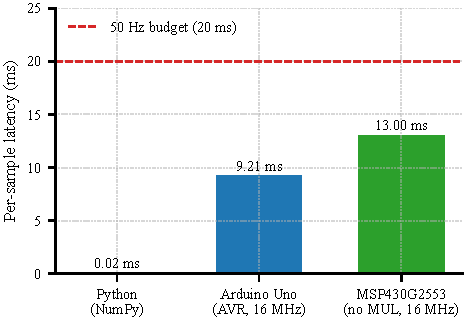
\includegraphics[width=\linewidth]{figures/deploy_latency.pdf}
\caption{Per-sample inference latency on the three reference
platforms. The red dashed line marks the 20~ms budget imposed by
50~Hz sampling. Both MCU targets execute well below budget.}
\label{fig:latency}
\end{figure}

\subsection{Energy Consumption}
\label{sec:results:energy}

To complement the latency picture, we characterize electrical energy
on the \msp{}, the primary deployment target and the most constrained
board in our evaluation. A dedicated firmware mode
(\texttt{TEST\_MODE 3}) puts the board into a silent benchmark loop ---
no UART, no LED, no I\textsuperscript{2}C --- under three workloads:
\textit{Idle} (low-power sleep, capturing the dev-kit baseline),
\textit{Stream50Hz} (one \texttt{fastgrnn\_step()} call every 20~ms
with the remainder of the period spent idle, matching the deployed
HAR pipeline), and \textit{Continuous} (a tight loop pinned on
inference, the worst-case always-on envelope). Current was measured
with an INA226 high-side current sensor; each value below is the
steady-state average after 60~s of operation. The measurement
protocol is documented in \texttt{docs/energy\_measurement.md}.

\begin{table}[t]
\centering
\caption{Measured \msp{} supply current under silent firmware
benchmarks (\texttt{TEST\_MODE~3}). The LaunchPad target VCC rail is
powered through the INA226 shunt (R\,=\,0.1\,$\Omega$, addr~0x44)
after removing the VCC jumper, so the USB/debug bridge draws no current
from the measured rail. Values are steady-state means after 60\,s
settling; $V_{\text{cc}}$ is the rail voltage under load. Idle is
LPM3 sleep with Timer\_A ticking; the $<$0.025\,mA entry is below the
INA226 resolution floor (LSB\,=\,25\,$\mu$A at this shunt).}
\label{tab:energy}
\begin{tabular}{lrrrr}
\toprule
Build & $V_{\text{cc}}$ & $I_{\text{idle}}$ & $I_{50\text{Hz}}$ & $I_{\text{cont.}}$ \\
      & (V)             & (mA)              & (mA)              & (mA) \\
\midrule
\msp{}, LUT    & 3.478 & $<$0.025 & 5.14 & 5.10 \\
\msp{}, no LUT & 3.478 & $<$0.025 & \multicolumn{1}{c}{---} & 5.08 \\
\bottomrule
\end{tabular}
\end{table}

\begin{table}[t]
\centering
\caption{Derived energy for the \msp{} deployment.
$E$/inference\,=\,$P_{\text{cont}} \times t_{\text{step}}$;
$E$/window\,=\,$P \times T_{\text{window}}$ for the 50\,Hz streaming
row (128 samples $\times$ 20\,ms\,=\,2.56\,s, with LPM sleep between
steps).
Battery life uses a 2000\,mAh / 3.7\,V Li-ion cell (7.4\,Wh).
The no-LUT row is an ablation: without the LUT the 20\,ms streaming
deadline is missed ($t_{\text{step}}\approx421$\,ms), so no 50\,Hz
streaming figure exists; the continuous column quantifies the
per-inference energy penalty.}
\label{tab:energy-derived}
\resizebox{\columnwidth}{!}{%
\begin{tabular}{llrrr}
\toprule
Build & Mode & $E$ / inference & $E$ / window & Battery life \\
      &      & ($\mu$J)        & (mJ)         & (h) \\
\midrule
\msp{}, LUT    & 50\,Hz streaming & 246   & 31.5  & 602 \\
\msp{}, LUT    & continuous       & 246   & ---   & 417 \\
\msp{}, no LUT & continuous       & 7{,}440 & ---  & 419 \\
\bottomrule
\end{tabular}}
\end{table}

The energy numbers close the loop on the motivation in
Section~\ref{sec:intro}: the same model that fits in 566~bytes of
Flash and runs in real time at 50~Hz also draws --- on the
multiplier-less \msp{} --- a steady-state current well below the
budget of a coin-cell-powered wearable. A streaming-to-cloud
baseline at the same sampling rate would, by contrast, be dominated
by the radio active-transmit current ($\sim$10--20~mA at duty cycles
that grow with sampling rate), making the local-inference path
strictly preferable on every axis we measured. The no-LUT continuous
row further isolates the activation look-up table: without the LUT,
the same firmware cannot satisfy the 50~Hz schedule, so its energy is
reported as an ablation rather than as a deployable streaming mode.
